\chapter{自分の研究本体を述べるところ}
ここは自分のやった研究を述べる章です。実際の中身に合わせて章を複数立てにする場合もあると思います。「議論」の章を別に分ける場合は、この章では得られた結果までを記述し、その結果に対する議論は「議論」の章に回すのが良いでしょう。この章は必ずしも1つの章のみである必要はありません。研究内容に応じて、複数の章に分割することも一般的に行われます。

\section{胃がんの画像データ取得方法}

\subsection{透明化と染色}
ホルマリン固定されている検体をLUCIDによる透明化してから染色する.
多光子顕微鏡で3D画像として撮影する.一つの視野で観察することができる領域は縦横が~で深さ方向が~である.ここでLUCIDによる透明化によって今までは断面のみの撮影だったものを深さ方向まで撮影することができるようになった.
検体全ての撮影をするために画像取得にはタイリングをする.

\begin{comment}

蛍光顕微鏡
Microscope name: Ti2 Microscope
Objective name: Plan Apo 10x
Objective magnification: 10
Objective numerical aperture: 0.45
Refractive Index: 1.000


レーザー波長の情報

DAPI
Emission wavelength: 440.0--420.0
Excitation wavelength: 405.0
Pinhole size: 20.00
Channel modality: Laser Scan Confocal, PMT

FITC
Emission wavelength: 500.0--550.0
Excitation wavelength: 405.0
Pinhole size: 20.00
Channel modality: Laser Scan Confocal, PMT

Texas Red
Emission wavelength: 593.0--670.0
Excitation wavelength: 561.0
Pinhole size: 20.00
Channel modality: Laser Scan Confocal, PMT

深さ方向の分解能
Z step : 2.7µm

\end{comment}


\tab {蛍光顕微鏡}に示すような蛍光顕微鏡で撮影を行った.また撮影条件を\tab {レーザー波長}にまとめた.

\begin{table}[H]
	\centering
	\caption{Information of fluorescence microscope}
	\label{tab:蛍光顕微鏡}
	\begin{tabular}{cc}\toprule
		Microscope name & Ti2 Microscope \\ 
		Objective name & Plan Apo 10x \\ 
		Objective magnification & 10 \\ 
		Objective numerical aperture & 0.45 \\ 
		Refractive Index & 1.000 \\
		Z step & 2.7 $\upmu$m \\ \bottomrule
	\end{tabular} 
\end{table}

\begin{table}[H]
	\centering
	\caption{Information of laser wavelength}
	\label{tab:レーザー波長}
	\begin{tabular}{cccc}\toprule
		& DAPI & FITC & Texas Red \\ \midrule
		Emission wavelength (nm) & 440.0--420.0 & 500.0--550.0 & 593.0--670.0 \\ 
		Excitation wavelength (nm) & 405.0 & 405.0 & 561.0 \\ 
		Pinhole size ($\upmu$m) & 20.00 & 20.00 & 20.00 \\ 
		Channel modality & \multicolumn{3}{c}{Laser Scan Confocal, PMT } \\ \bottomrule
	\end{tabular}
\end{table}




% 三次元に撮影した画像

\begin{figure}[H]
	\centering
	
	\begin{minipage}{0.45\columnwidth}
		\centering
		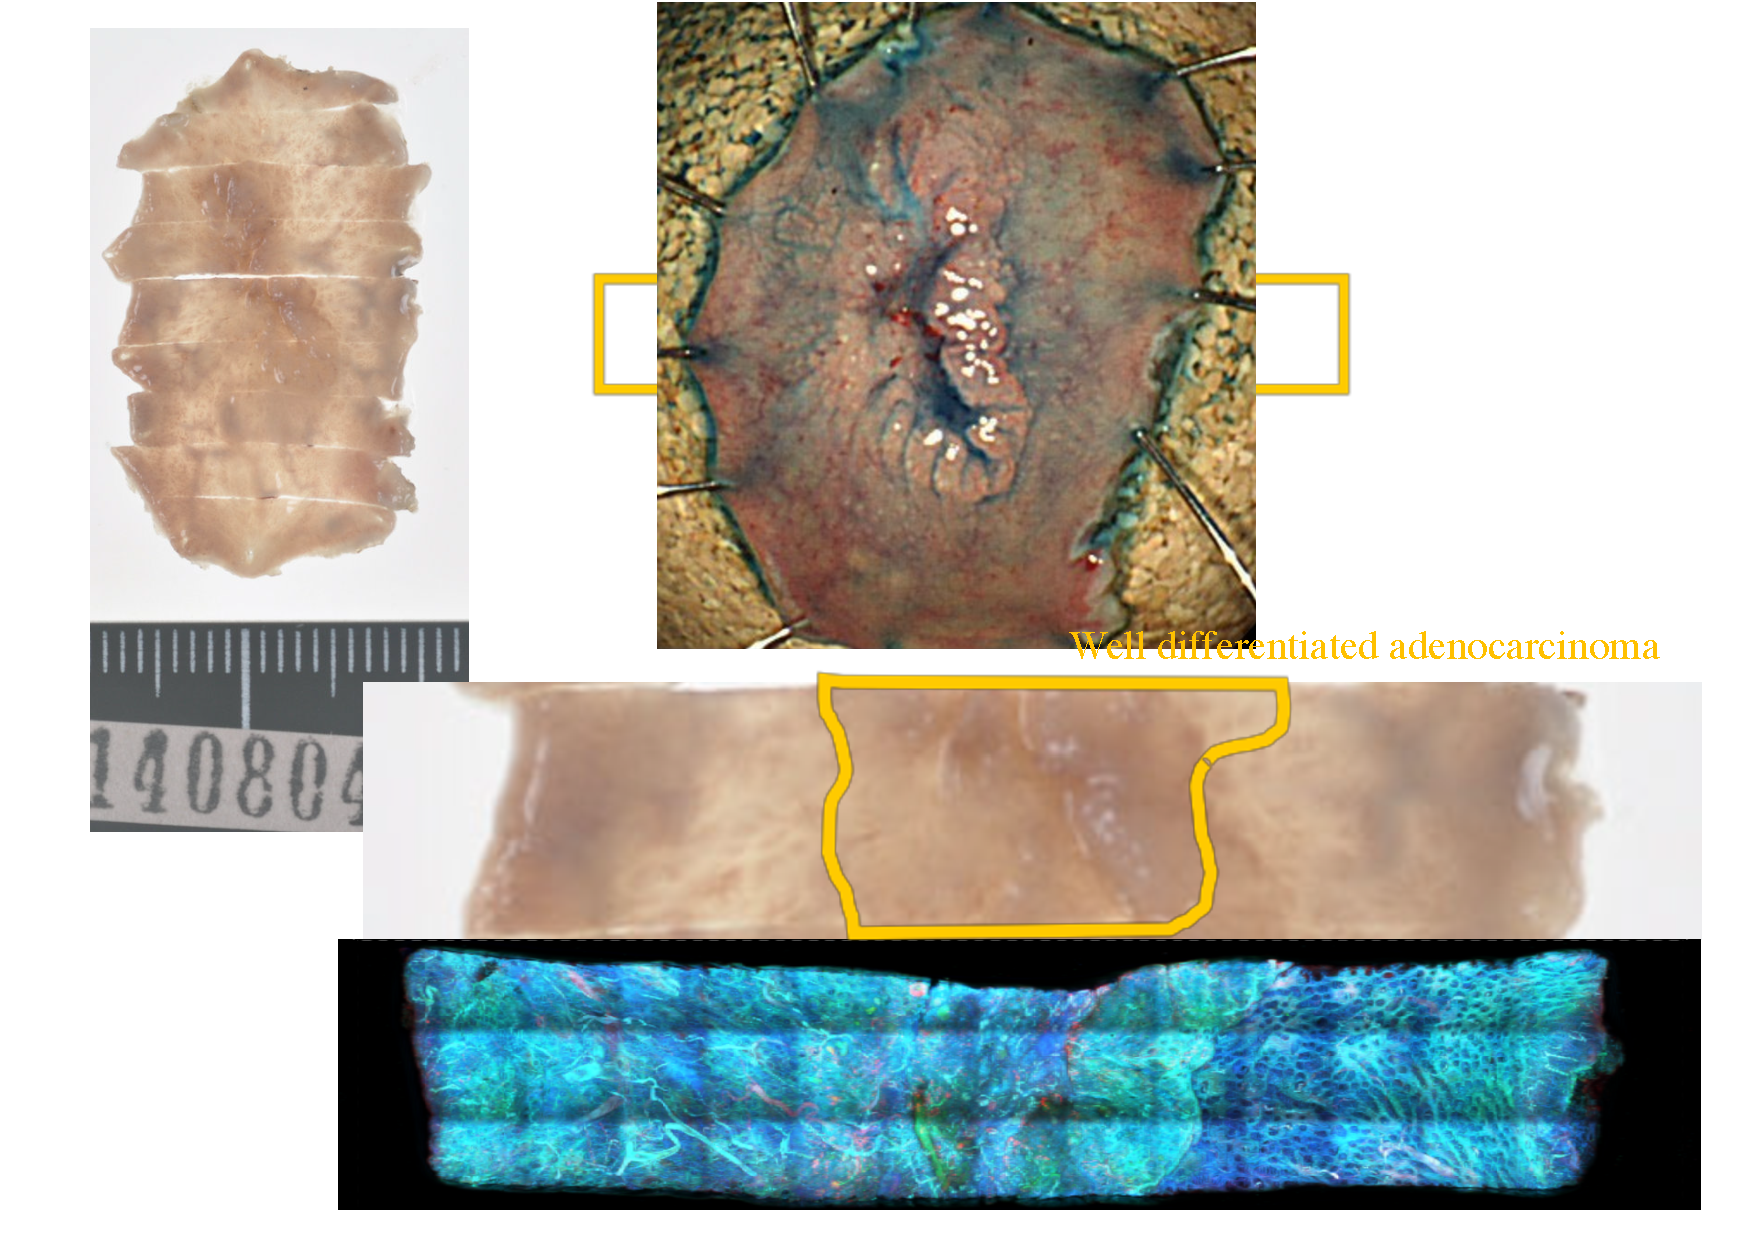
\includegraphics[clip, angle=270, width=\linewidth]{fig/raw_data/summary/C-013}
		\subcaption{sample A}
	\end{minipage}
	\begin{minipage}{0.45\linewidth}
		\centering
		%	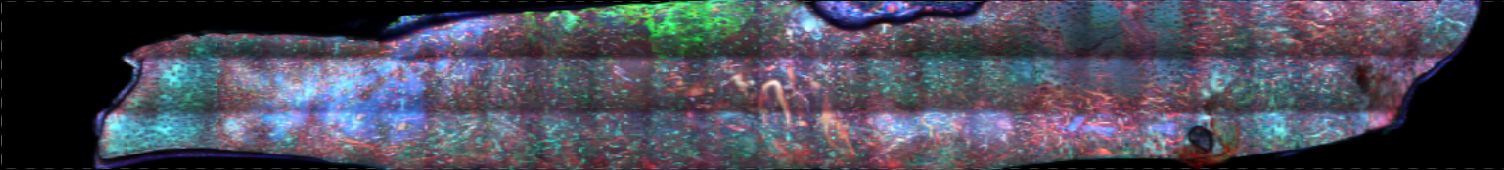
\includegraphics[clip, angle=270, width=\linewidth]{fig/raw_data/summary/C-012}
		\subcaption{sample B}
	\end{minipage}
	\begin{minipage}{0.45\columnwidth}
		\centering
		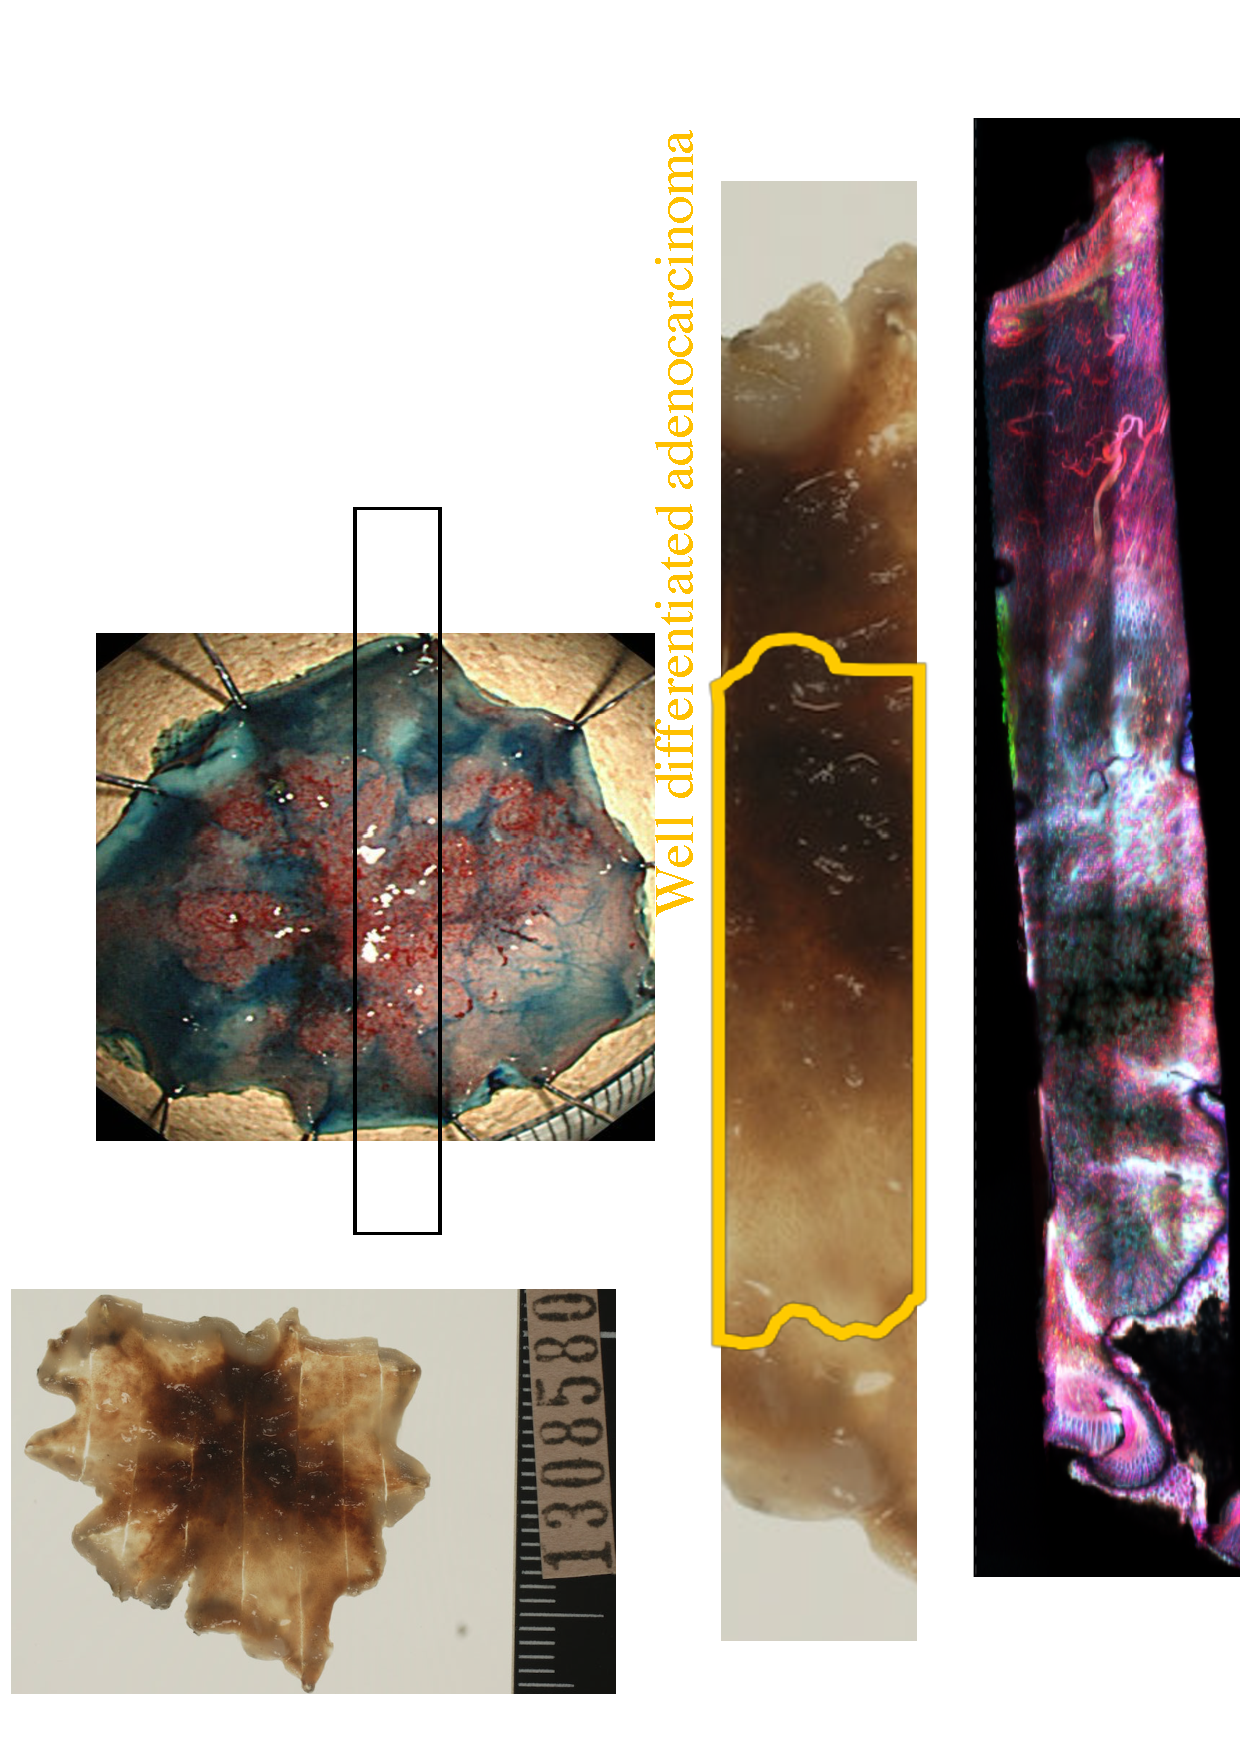
\includegraphics[clip, angle=270, width=\linewidth]{fig/raw_data/summary/C-009}
		\subcaption{sample C}
	\end{minipage}
	\begin{minipage}{0.45\linewidth}
		\centering
		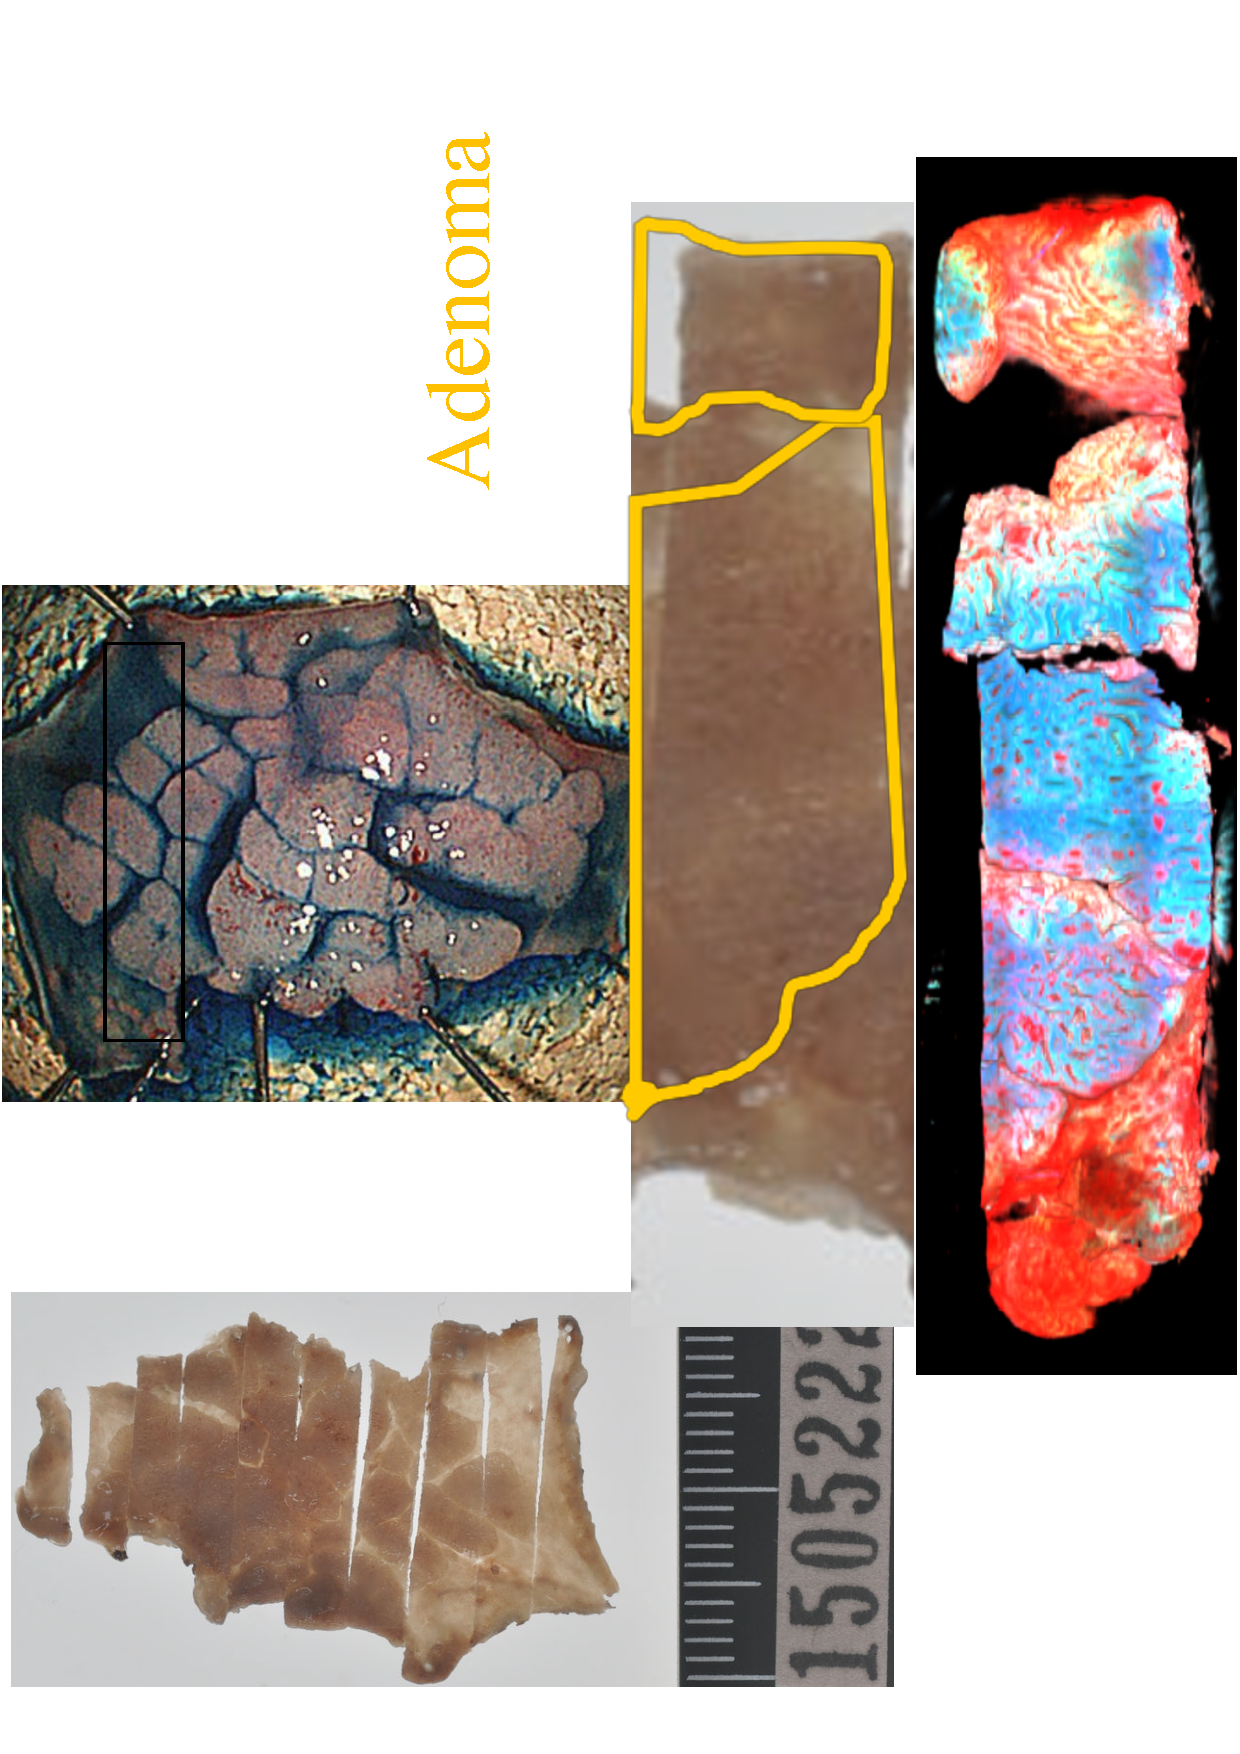
\includegraphics[clip, angle=270, width=\linewidth]{fig/raw_data/summary/C-011}
		\subcaption{sample D}
	\end{minipage}
	
	\caption{Overview samples}
	\label{fig:検体一覧}
	
\end{figure}


\subsection{教師データの作成}
消化器内科の医師がつけた腫瘍部分を教師データとして利用した.\fig {コラ画像}が腫瘍の位置をマスクした画像になっている.

\begin{figure}[H]
	\centering
	
	\begin{minipage}{0.8\columnwidth}
		\centering
		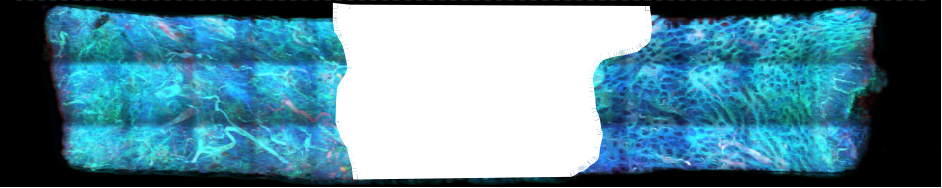
\includegraphics[clip, width=\linewidth]{fig/raw_data/label/C-013}
		\subcaption{sample A}
	\end{minipage}	
	
	\begin{minipage}{0.8\columnwidth}
		\centering
		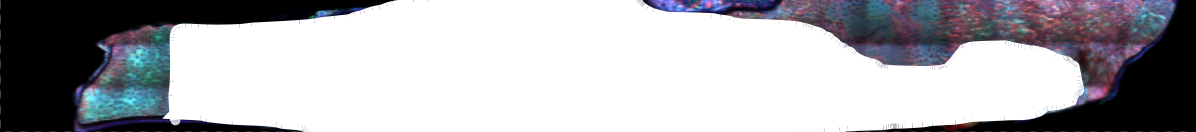
\includegraphics[clip, width=\linewidth]{fig/raw_data/label/C-012}
		\subcaption{sample B}
	\end{minipage}
	
	\begin{minipage}{0.8\columnwidth}
		\centering
		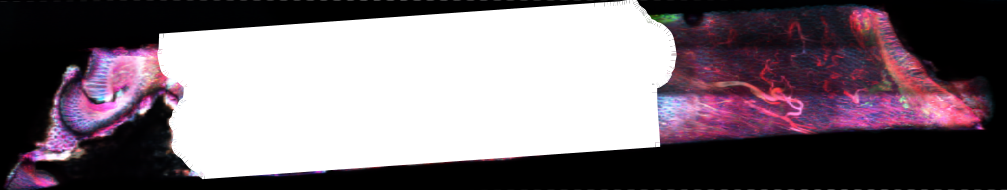
\includegraphics[clip, width=\linewidth]{fig/raw_data/label/C-009}
		\subcaption{sample C}
	\end{minipage}
	
	\begin{minipage}{0.8\columnwidth}
		\centering
		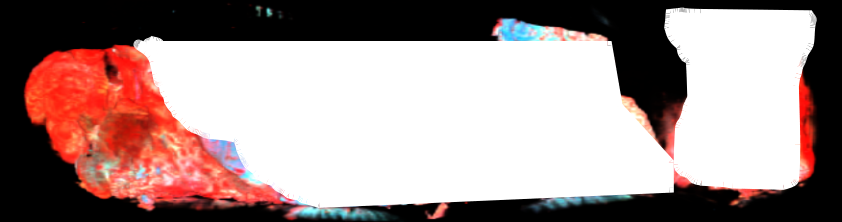
\includegraphics[clip, width=\linewidth]{fig/raw_data/label/C-011}
		\subcaption{sample D}
	\end{minipage}
	%\begin{minipage}{0.8\columnwidth}
	%	\centering
	%	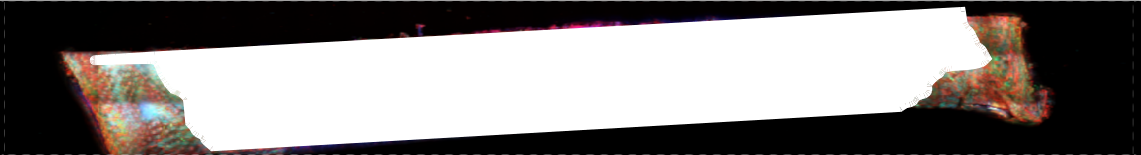
\includegraphics[clip, width=\linewidth]{fig/raw_data/label/C-010}
	%	\subcaption{sample E}
	%\end{minipage}
	
	\caption{Sample images masking cancer}
	\label{fig:コラ画像}
	
\end{figure}


\section{前処理}

\subsection{擬似HE染色}
\begin{figure}[H]
	\centering
	
	\begin{minipage}{0.8\columnwidth}
		\centering
		\includegraphics[clip, angle=270, width=\linewidth]{fig/preprocessing/pseudo-HE/0130171}
		\subcaption{sample A}
	\end{minipage}
	\begin{minipage}{0.8\columnwidth}
		\centering
		\includegraphics[clip, angle=270, width=\linewidth]{fig/preprocessing/pseudo-HE/0120100}
		\subcaption{sample B}
	\end{minipage}
	\begin{minipage}{0.8\columnwidth}
		\centering
		\includegraphics[clip, angle=270, width=\linewidth]{fig/preprocessing/pseudo-HE/201901150050}
		\subcaption{sample C}
	\end{minipage}
	\begin{minipage}{0.8\columnwidth}
		\centering
		\includegraphics[clip, angle=270, width=\linewidth]{fig/preprocessing/pseudo-HE/0110240}
		\subcaption{sample D}
	\end{minipage}
	
	%\begin{minipage}{0.8\columnwidth}
	%	\centering
	%	\includegraphics[clip, angle=270, width=\linewidth]{fig/preprocessing/pseudo-HE/0100}
	%	\subcaption{sample E}
	%\end{minipage}
	
	\caption{Sample images preprocessing like HE}
	\label{fig:HElike}
	
\end{figure}


教師ラベルから,正常と腫瘍に分割した.
\begin{figure}[H]
	\centering
	
	\begin{minipage}{0.4\columnwidth}
		\centering
		\includegraphics[clip, width=\linewidth]{fig/preprocessing/separated_label/normal/normal_C-013}
		\subcaption{Normal of sample A}
	\end{minipage}
	\begin{minipage}{0.4\columnwidth}
		\centering
		\includegraphics[clip, width=\linewidth]{fig/preprocessing/separated_label/cancer/cancer_C-013}
		\subcaption{Cancer of sample A}
	\end{minipage}
	
	\caption{Teacher labels of normal and cancer}
	\label{fig:検体A教師ラベル}
	
\end{figure}

\subsection{Data Augmentation}
本研究では少量のデータセットであるため,少しの画像からより多くの特徴を抽出するために擬似的にデータの水増し(Data Augmentation)を行った.本研究で注意した点は,入力画像としてあり得る範囲のバリエーションに絞った点である.

\subsection*{回転}

\begin{figure}[H]
	\centering
	
	\begin{minipage}{0.24\columnwidth}
		\centering
		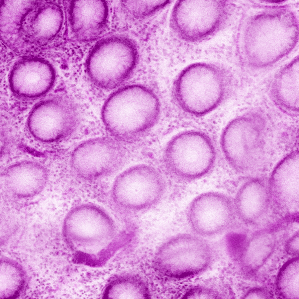
\includegraphics[clip, width=\linewidth]{fig/preprocessing/data_aug/rotate/ROTATION_0}
		\subcaption{0\deg}
	\end{minipage}
	\begin{minipage}{0.24\columnwidth}
		\centering
		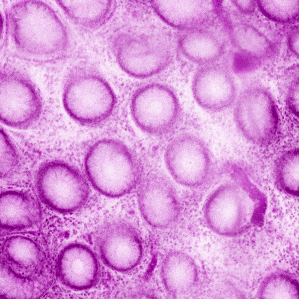
\includegraphics[clip, width=\linewidth]{fig/preprocessing/data_aug/rotate/ROTATION_90}
		\subcaption{90\deg}
	\end{minipage}
	\begin{minipage}{0.24\columnwidth}
		\centering
		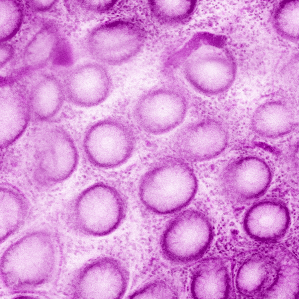
\includegraphics[clip, width=\linewidth]{fig/preprocessing/data_aug/rotate/ROTATION_180}
		\subcaption{180\deg}
	\end{minipage}
	\begin{minipage}{0.24\columnwidth}
		\centering
		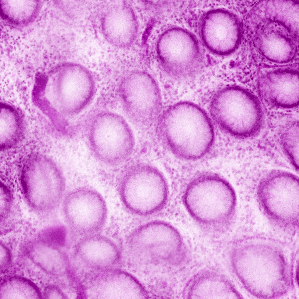
\includegraphics[clip, width=\linewidth]{fig/preprocessing/data_aug/rotate/ROTATION_270}
		\subcaption{270\deg}
	\end{minipage}
	
	\caption{Rotation}
	\label{fig:回転}
	
\end{figure}


\subsection*{反転}

\begin{figure}[H]
	\centering
	
	\begin{minipage}{0.25\columnwidth}
		\centering
		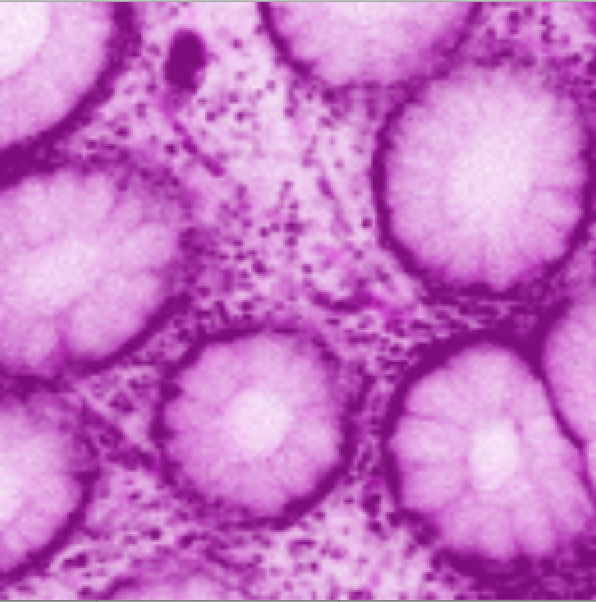
\includegraphics[clip, width=\linewidth]{fig/preprocessing/data_aug/horizontal_flip/horizontal_flip}
		\subcaption{horizontal flipping}
	\end{minipage}
	\begin{minipage}{0.1\columnwidth}
		\hspace{2truemm}
	\end{minipage}
	\begin{minipage}{0.25\columnwidth}
		\centering
		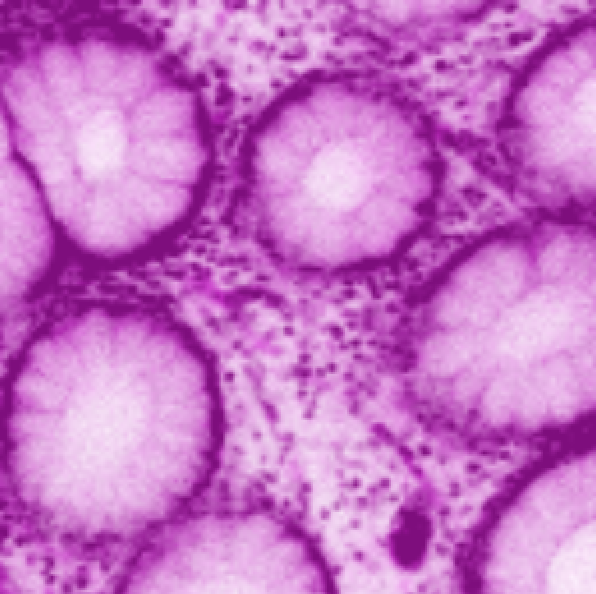
\includegraphics[clip, width=\linewidth]{fig/preprocessing/data_aug/vertical_flip/vertical_flip}
		\subcaption{vertical flipping}
	\end{minipage}
	
	\caption{Flipping}
	\label{fig:反転}
	
\end{figure}

\subsection*{ガウシアンブラー}

\begin{figure}[H]
	\centering
	
	\begin{minipage}{0.24\columnwidth}
		\centering
		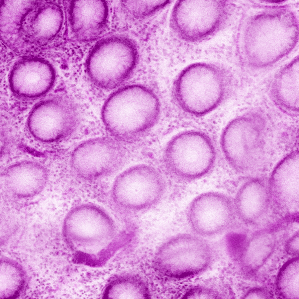
\includegraphics[clip, width=\linewidth]{fig/preprocessing/data_aug/color/blur/blur_0_00}
		\subcaption{$r=0$}
	\end{minipage}
	\begin{minipage}{0.24\columnwidth}
		\centering
		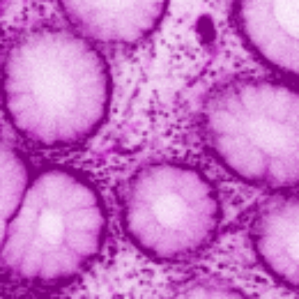
\includegraphics[clip, width=\linewidth]{fig/preprocessing/data_aug/color/blur/blur_0_50}
		\subcaption{$r=0.50$}
	\end{minipage}
	\begin{minipage}{0.24\columnwidth}
		\centering
		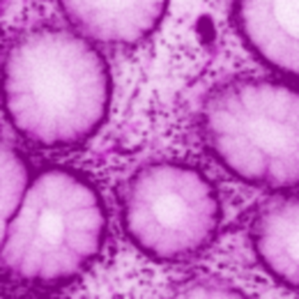
\includegraphics[clip, width=\linewidth]{fig/preprocessing/data_aug/color/blur/blur_1_00}
		\subcaption{$r=1.00$}
	\end{minipage}
	\begin{minipage}{0.24\columnwidth}
		\centering
		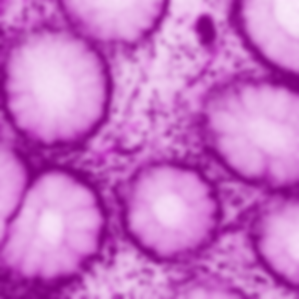
\includegraphics[clip, width=\linewidth]{fig/preprocessing/data_aug/color/blur/blur_2_00}
		\subcaption{$r=2.00$}
	\end{minipage}
	
	\caption{Gaussian blur. $r$ is blur radius.}
	\label{fig:ガウシアンブラー}
	
\end{figure}

\subsection*{鮮鋭度}

\begin{figure}[H]
	\centering
	
	\begin{minipage}{0.24\columnwidth}
		\centering
		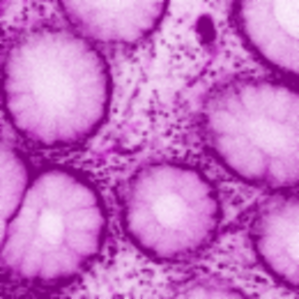
\includegraphics[clip, width=\linewidth]{fig/preprocessing/data_aug/color/SHARPNESS/SHARPNESS_0_00}
		\subcaption{$f=0$}
	\end{minipage}
	\begin{minipage}{0.24\columnwidth}
		\centering
		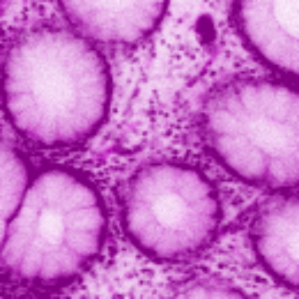
\includegraphics[clip, width=\linewidth]{fig/preprocessing/data_aug/color/SHARPNESS/SHARPNESS_0_50}
		\subcaption{$f=0.50$}
	\end{minipage}
	\begin{minipage}{0.24\columnwidth}
		\centering
		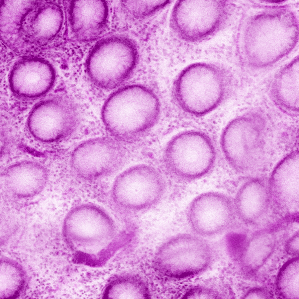
\includegraphics[clip, width=\linewidth]{fig/preprocessing/data_aug/color/SHARPNESS/SHARPNESS_1_00}
		\subcaption{$f=1.00$}
	\end{minipage}
	\begin{minipage}{0.24\columnwidth}
		\centering
		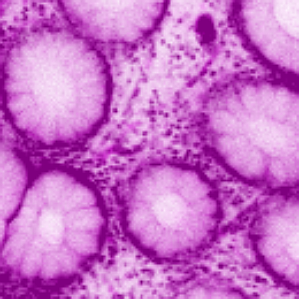
\includegraphics[clip, width=\linewidth]{fig/preprocessing/data_aug/color/SHARPNESS/SHARPNESS_2_00}
		\subcaption{$f=2.00$}
	\end{minipage}
	
	\caption{Sharpness. $f$ is enhancement factor. An enhancement factor of 0.0 gives a blurred image, a factor of 1.0 gives the original image, and a factor of 2.0 gives a sharpened image.}
	\label{fig:シャープネス}
	
\end{figure}

\subsection*{輝度}
\begin{figure}[H]
	\centering
	
	\begin{minipage}{0.25\columnwidth}
		\centering
		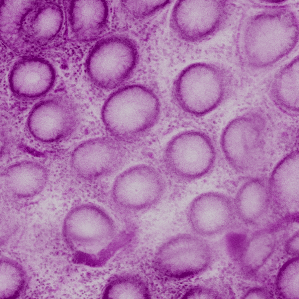
\includegraphics[clip, width=\linewidth]{fig/preprocessing/data_aug/color/BRIGHTNESS/BRIGHTNESS_0_80}
		\subcaption{$I=0.80$}
	\end{minipage}
	\begin{minipage}{0.25\columnwidth}
		\centering
		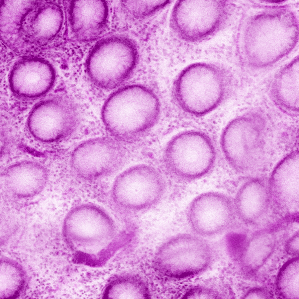
\includegraphics[clip, width=\linewidth]{fig/preprocessing/data_aug/color/BRIGHTNESS/BRIGHTNESS_1_00}
		\subcaption{$I=1.00$}
	\end{minipage}
	\begin{minipage}{0.25\columnwidth}
		\centering
		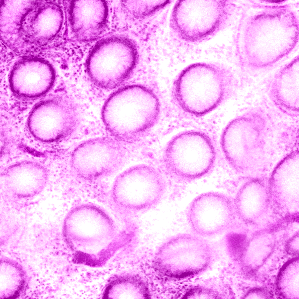
\includegraphics[clip, width=\linewidth]{fig/preprocessing/data_aug/color/BRIGHTNESS/BRIGHTNESS_1_20}
		\subcaption{$I=1.20$}
	\end{minipage}
	
	\caption{Intensity. $I$ is intensity of RGB color. An intensity of 0.0 gives a black image. An intensity of 1.0 gives the original image.}
	\label{fig:輝度}
	
\end{figure}

\subsection*{コントラスト}
\begin{figure}[H]
	\centering
	
	\begin{minipage}{0.25\columnwidth}
		\centering
		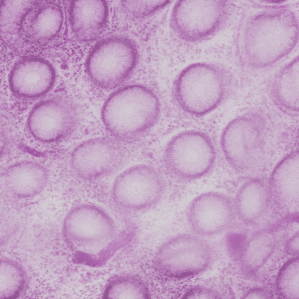
\includegraphics[clip, width=\linewidth]{fig/preprocessing/data_aug/color/CONTRAST/CONTRAST_0_50}
		\subcaption{$f = 0.50$}
	\end{minipage}
	\begin{minipage}{0.25\columnwidth}
		\centering
		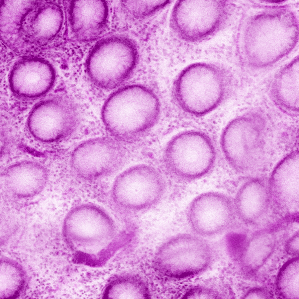
\includegraphics[clip, width=\linewidth]{fig/preprocessing/data_aug/color/CONTRAST/CONTRAST_1_00}
		\subcaption{$f = 1.00$}
	\end{minipage}
	\begin{minipage}{0.25\columnwidth}
		\centering
		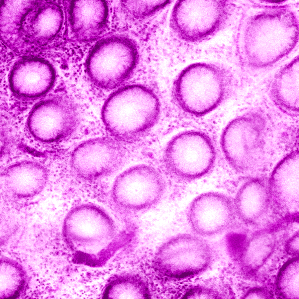
\includegraphics[clip, width=\linewidth]{fig/preprocessing/data_aug/color/CONTRAST/CONTRAST_1_50}
		\subcaption{$f = 1.50$}
	\end{minipage}	
	
	\caption{Contrast. $f$ is enhancement factor. An enhancement factor of 0.0 gives a solid grey image. A factor of 1.0 gives the original image.}
	\label{fig:}
	
\end{figure}

\subsection*{彩度}
\begin{figure}[H]
	\centering
	
	\begin{minipage}{0.25\columnwidth}
		\centering
		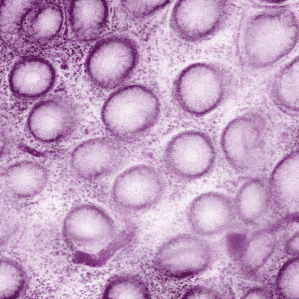
\includegraphics[clip, width=\linewidth]{fig/preprocessing/data_aug/color/SATURATION/SATURATION_0_50}
		\subcaption{$f = 0.50$}
	\end{minipage}
	\begin{minipage}{0.25\columnwidth}
		\centering
		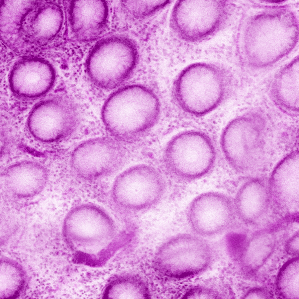
\includegraphics[clip, width=\linewidth]{fig/preprocessing/data_aug/color/SATURATION/SATURATION_1_00}
		\subcaption{$f = 1.00$}
	\end{minipage}
	\begin{minipage}{0.25\columnwidth}
		\centering
		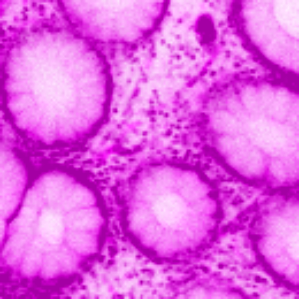
\includegraphics[clip, width=\linewidth]{fig/preprocessing/data_aug/color/SATURATION/SATURATION_1_50}
		\subcaption{$f = 1.50$}
	\end{minipage}	
	
	\caption{Saturation. $f$ is enhancement factor. An enhancement factor of 0.0 gives a black and white image. A factor of 1.0 gives the original image.}
	\label{fig:彩度}
	
\end{figure}

\subsection{クロッピング画像}

\begin{figure}[H]
	\centering
	
	\begin{minipage}{0.45\columnwidth}
		\centering
		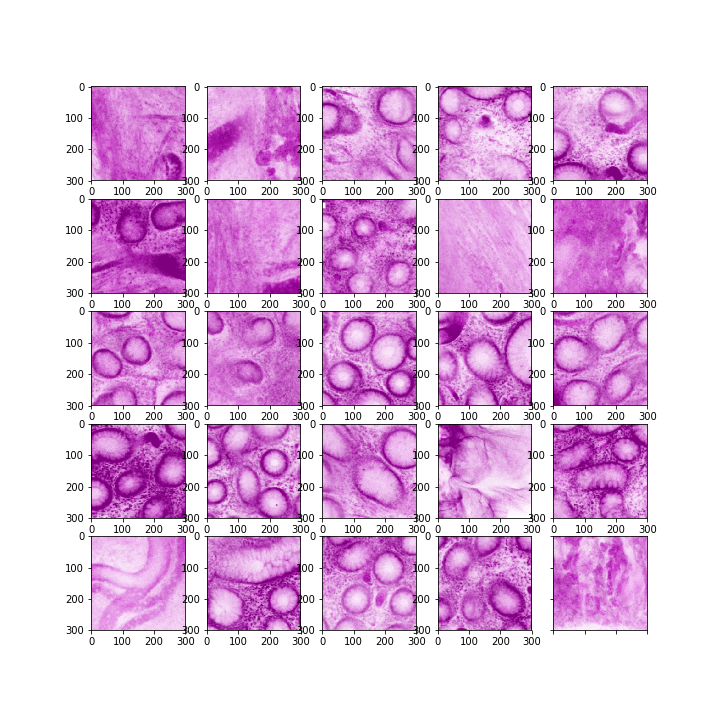
\includegraphics[clip, width=\linewidth]{fig/preprocessing/cropping/HE/normal/C-013}
		\subcaption{Normal images of sample A}
	\end{minipage}
	\begin{minipage}{0.45\columnwidth}
		\centering
		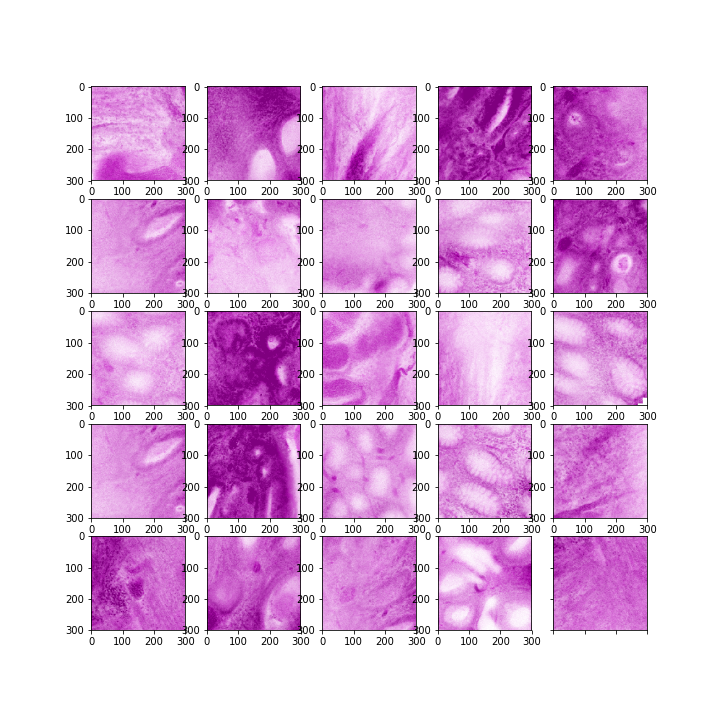
\includegraphics[clip, width=\linewidth]{fig/preprocessing/cropping/HE/cancer/C-013}
		\subcaption{Cancer images of sample A}
	\end{minipage}
	
	\begin{minipage}{0.45\columnwidth}
		\centering
		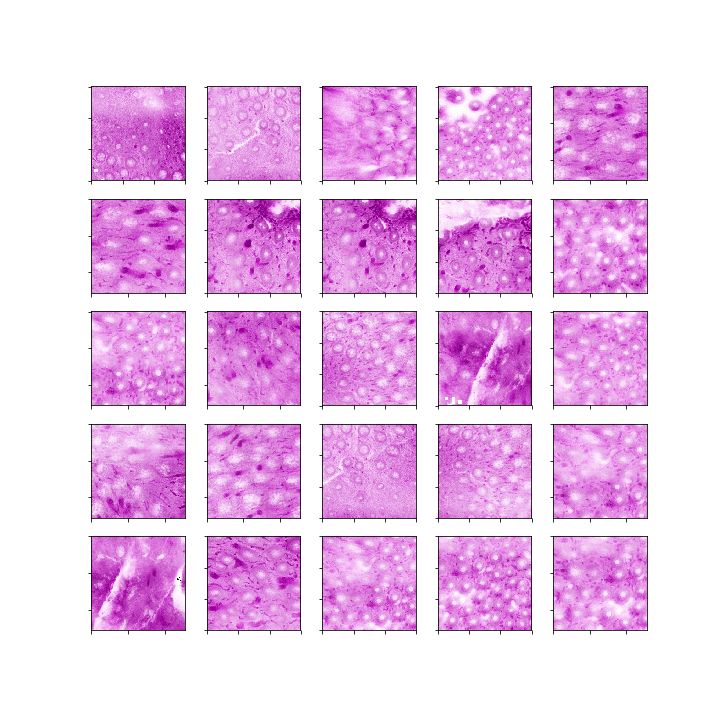
\includegraphics[clip, width=\linewidth]{fig/preprocessing/cropping/HE/normal/C-012}
		\subcaption{Normal images of sample B}
	\end{minipage}
	\begin{minipage}{0.45\columnwidth}
		\centering
		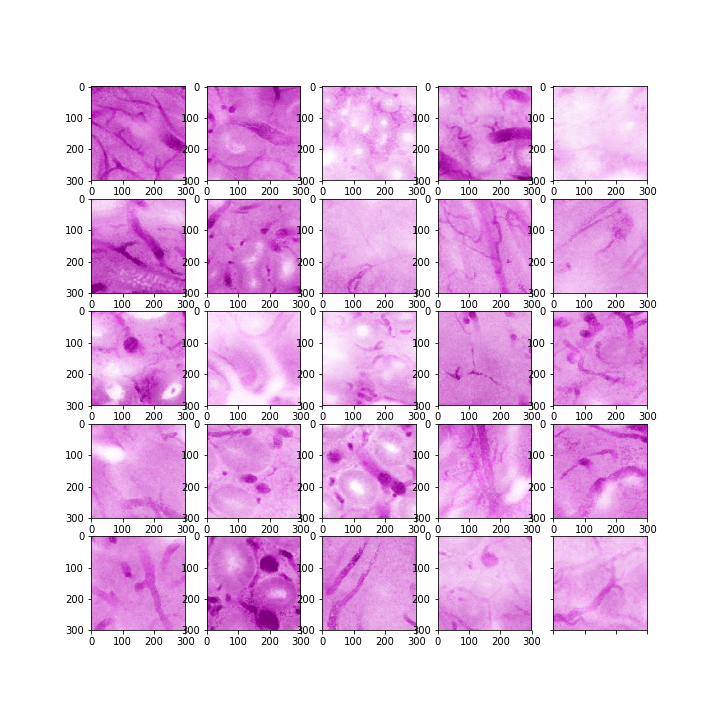
\includegraphics[clip, width=\linewidth]{fig/preprocessing/cropping/HE/cancer/C-012}
		\subcaption{Cancer images of sample B}
	\end{minipage}
	
	\caption{Cropped images for validation}
	\label{fig:クロップ}
	
\end{figure}

\section{古典的な画像処理手法による識別精度評価}
正常と腫瘍を両方含む画像に対してHough変換による円検出で正常の線管構造を検出した.円検出では検出できない線菅構造をより多く検出するために楕円でも検出ができるように変更した.複数のパラメータを調整することで,アノテーションの正常領域が検出できるような円検出の数を増やしながらも,ノイズが多くならないような値を決定した.また,これが複数の検体で試してみた時に,最適なパラメータを見積もった.

\section{事前学習}
今回のように新しい画像の撮影方法でデータを多く集めることができない時は,類似データを事前に学習しておく事前学習を用いる.
大腸の管構造の特徴を捉えるために,外部のデータセットのGland Challengeデータセットを使って事前学習を行う.

\begin{tabular}{|cc}
	\hline 
	Cancer Type & Colorectal Cancer \\ 
	\hline 
	Resolution & $20X (0.62005 \mu{m}/pixel)$ \\ 
	\hline 
	Number
	
	of Images & 165 \\ 
	\hline 
	Format & bmp \\ 
	\hline 
\end{tabular} 

\begin{figure}[H]
	\centering
	
	\begin{minipage}{0.45\columnwidth}
		\centering
		\includegraphics[clip, width=\linewidth]{fig/chapter2/pretrain_image/testA_5.bmp}
		\subcaption{Normal images of sample A}
	\end{minipage}
	\begin{minipage}{0.45\columnwidth}
		\centering
		\includegraphics[clip, width=\linewidth]{fig/chapter2/pretrain_image/testA_35.bmp}
		\subcaption{Cancer images of sample A}
	\end{minipage}
	
	\begin{minipage}{0.45\columnwidth}
		\centering
		\includegraphics[clip, width=\linewidth]{fig/chapter2/pretrain_image/testA_12.bmp}
		\subcaption{Normal images of sample B}
	\end{minipage}
	\begin{minipage}{0.45\columnwidth}
		\centering
		\includegraphics[clip, width=\linewidth]{fig/chapter2/pretrain_image/train_77.bmp}
		\subcaption{Cancer images of sample B}
	\end{minipage}
	
	\caption{Cropped images for validation}
	\label{fig:事前学習画像}
	
\end{figure}

画像サイズが(755, 522)である枚数が151枚であり,それ以外は使用しなかった.

\section{教師あり学習による識別精度評価}
% モデルの概略図

\subsection{評価方法}
機械学習の評価方法には,ホールドアウト法と交差検証法の2通りある.ホールドアウト法はデータを訓練データとテストデータに分割して評価する方法である.交差検証法はデータをK分割してK-1のグループを訓練データに,残りの1つをテストデータにする.これをKパターン全て試行した精度の平均で評価する方法である.交差検証法の方が計算時間が長くなるが信頼性が高い.少量のデータの場合は特に訓練データとテストデータの分割の違いで結果に差が生じることがあるため本研究の評価方法では交差検証法を用いた.

本研究では4検体を使っているため検体ごとに分割することで4分割の交差検証法を行った.

\subsection*{2次元画像}
用いたネットワーク構造は,InceptionV3, Xception, Inception\_Resnetの4つである
それぞれに対して,Data Augmentation,事前学習,擬似HE染色のありなしで精度がどのように改善されるかを実験した.

\subsection*{3次元画像}
深さ方向の15枚をまとめて3次元画像として解析する.
用いたモデルは3DCNN, Stacked CNN, 2DCNN\_LSTMである.
ここでは,Data Augmentationと事前学習と擬似HE染色は,全て適用して実験を行った.

\section{教師なし学習による識別精度評価}
Auto Encoder, GAN, VAE, VAE-GANで教師なし学習を行った.

\section{半教師あり学習による識別精度評価}
VAEの考えを利用して,半教師あり学習のネットワークを作成した.
\begin{figure}[H]
	\centering
	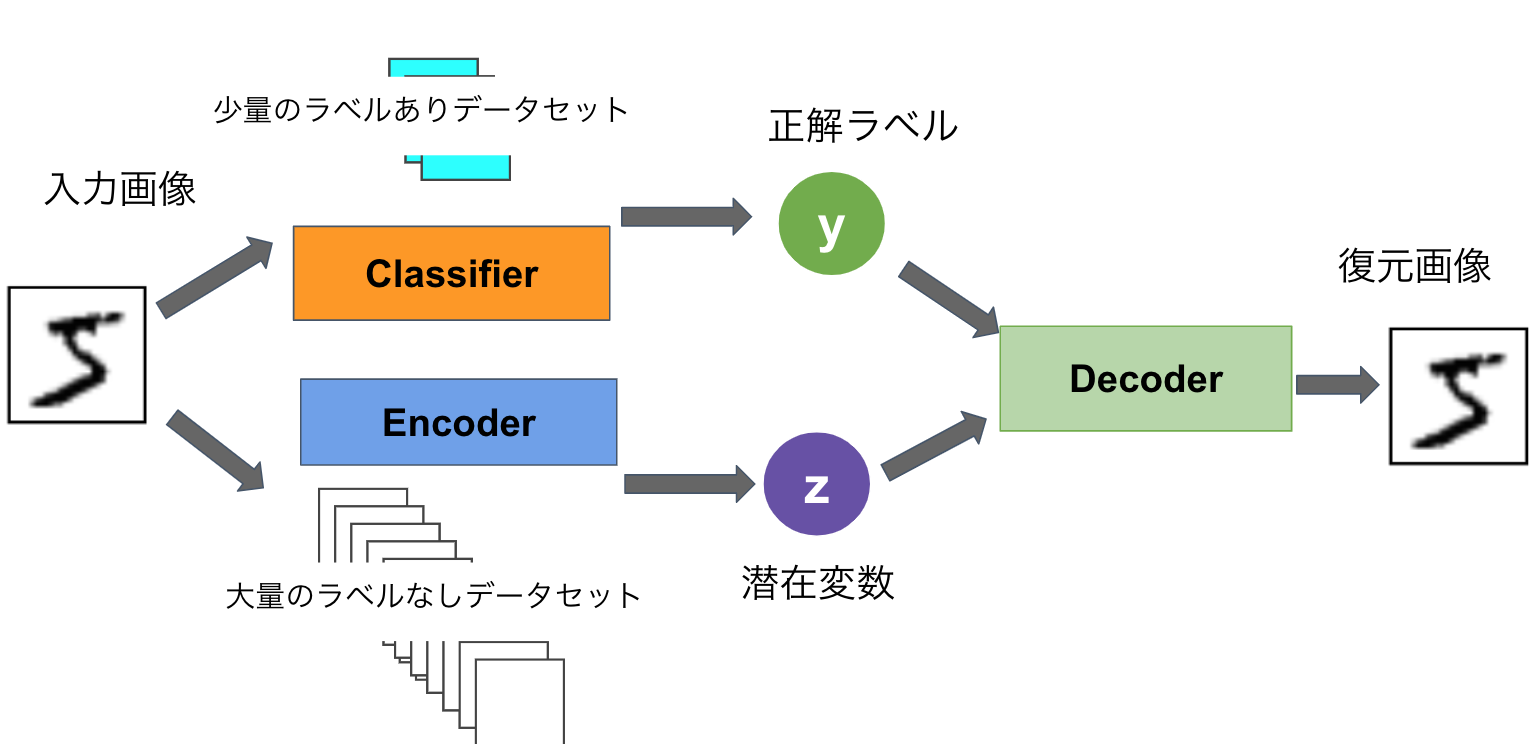
\includegraphics[width=0.7\linewidth]{fig/chapter3/networks/patern_A}
	\caption{}
	\label{fig:paterna}
\end{figure}

\begin{figure}[H]
	\centering
	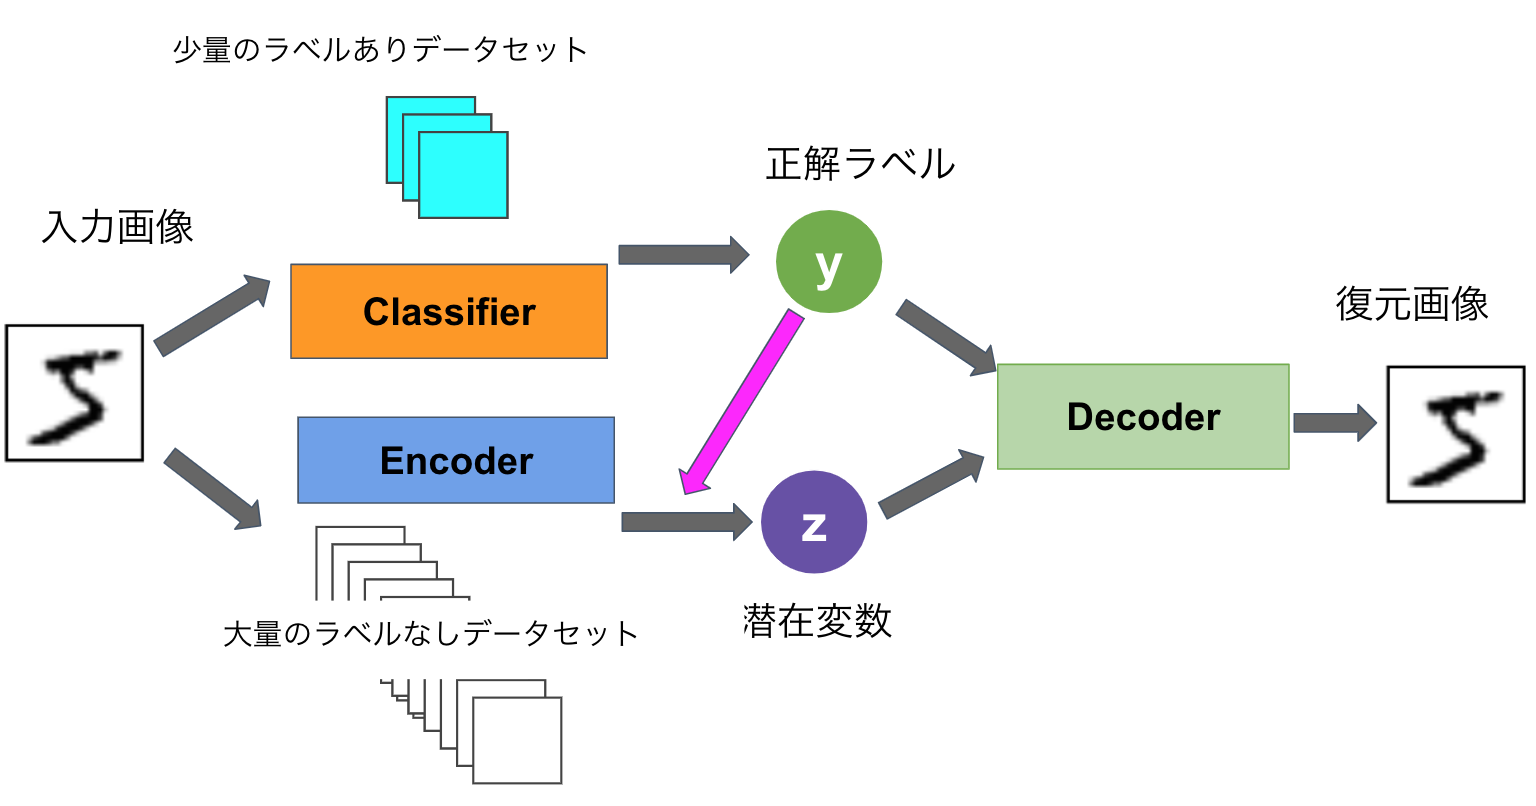
\includegraphics[width=0.7\linewidth]{fig/chapter3/networks/patern_B}
	\caption{}
	\label{fig:paterna}
\end{figure}


\section{学習環境}
\begin{table}[H]
	\centering
	\caption{Enviroment of implementation}
	\label{tab:環境}
	\begin{tabular}{ccc}\toprule
		OS & Ubuntu & ver. 14.04 \\ 
		Language & Python & ver. 3.6 \\ 
		\multirow{2}{*}{Framework} & Keras & ver. 2.2.4 \\ 
		& Tensorflow & ver. 1.11.0 \\ 
		GPU & GeForceRX 1080Ti & $\times$3 \\  \bottomrule
	\end{tabular}
\end{table}

Githubにコードを上げてある.
URL : 
